\documentclass[12pt,a4paper]{article}
\usepackage[utf8]{inputenc}
\usepackage[english]{babel}
\usepackage[T1]{fontenc}
\usepackage{amsmath}
\usepackage{amsfonts}
\usepackage{amssymb}
\usepackage{graphicx}
\usepackage{siunitx}
\usepackage{float}
\usepackage[left=2cm,right=2cm,top=2cm,bottom=2cm]{geometry}
\author{Gerald}

\begin{document}
\sisetup{separate-uncertainty = true}
	\setlength{\parindent}{0pt} 
	\begin{center}
		{\LARGE Experiment protocol}\\
		\begin{large}
			for the solid state lab course\\[0.4cm]
			at RWTH Aachen\\
			II. Physikalisches Institut A\\[5.5cm]
			\Large\textbf{\textsl{Superconductivity and SQUID}}\\[5.5cm]
			\normalsize\textit{authored\\by}\\[0.4cm]
			\large{Moritz Berger (355244)\\Gerald Kolter (355005)}\\[2cm]
			\large \textbf{Summer term 2019}
		\end{large}
	\end{center}
	\newpage
	
	\tableofcontents
	\newpage

\section{Impact of the Laser wavelength}
The encapsulated graphene is used to analyze the impact of the Laser wavelength on the Raman spectrum. The $\omega_g$ vs. $\omega_{2D}$ map is shown in figure \ref{fig:Laser_omega} for both Lasers. The distribution of the individual positions are also shown in figure \ref{fig:Laser_omega_hist}.\\
The $\omega_g$ position is not shifted at all. However the $\omega_{2D}$ position shifted from an average position of \SI{2719(3)}{cm^{-1}} for the blue laser to \SI{2683(3)}{cm^{-1}} for the green laser. The reason for this is that only a single electron/hole site participates in the Raman process that leads to the G-line. By changing the Laser frequency only the excitation energy changes. The Raman shift stay the same. The 2D-line requires two lattice sites and the phonon modes connect them. Changing the excitation energy also changes the phonon modes and with that the Raman shift.\\

\begin{figure}
\centering
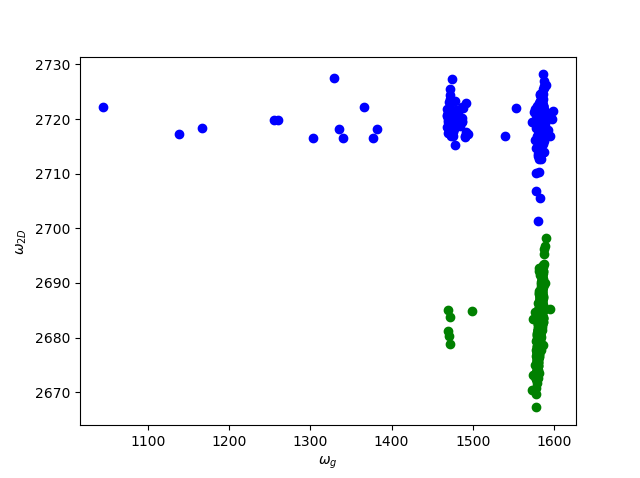
\includegraphics[scale=0.5]{Bilder/Laser/omega.png}
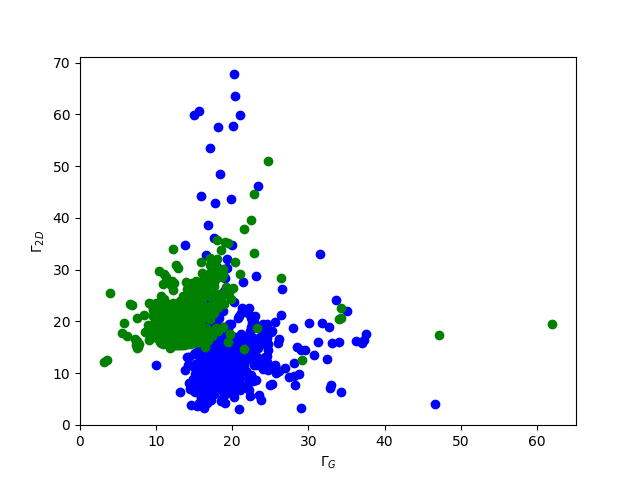
\includegraphics[scale=0.5]{Bilder/Laser/gamma.png}
\caption{line data of the G-line plotted against the 2D-line for both Lasers. Left: $\omega$, right: $\Gamma$. The Data point of the green laser are plotted in green and the blue laser in blue.}
\label{fig:Laser_omega}
\end{figure}

\begin{figure}
\centering
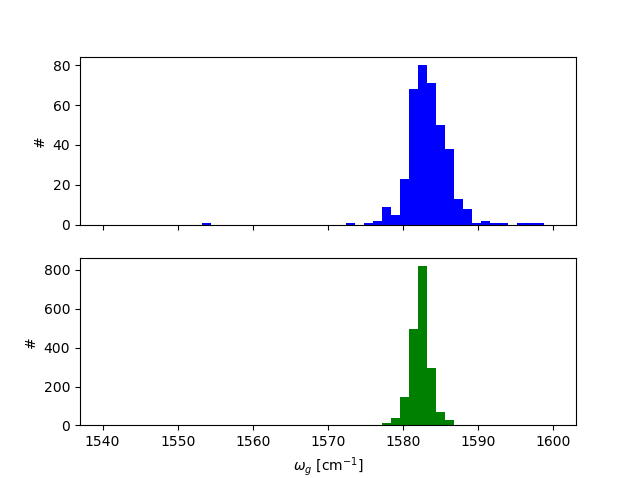
\includegraphics[scale=0.5]{Bilder/Laser/omegag_hist.png}
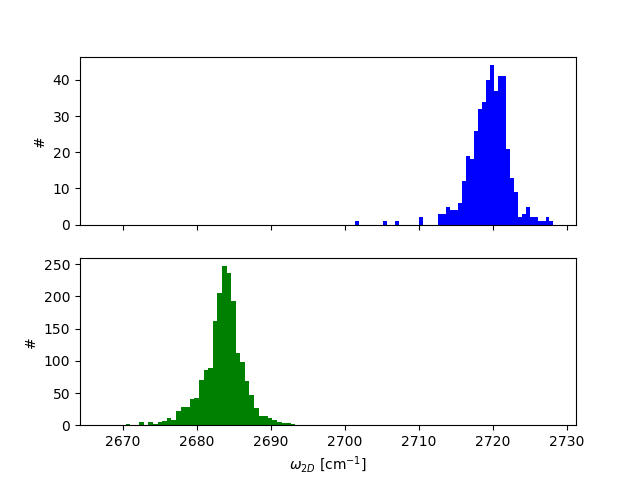
\includegraphics[scale=0.5]{Bilder/Laser/omega2d_hist.png}
\caption{Distribution of the line positions for the blue(top) and green(bottom) Laser. Right: $\omega_{g}$, left: $\omega_{2D}$.}
\label{fig:Laser_omega_hist}
\end{figure}

\begin{figure}
\centering
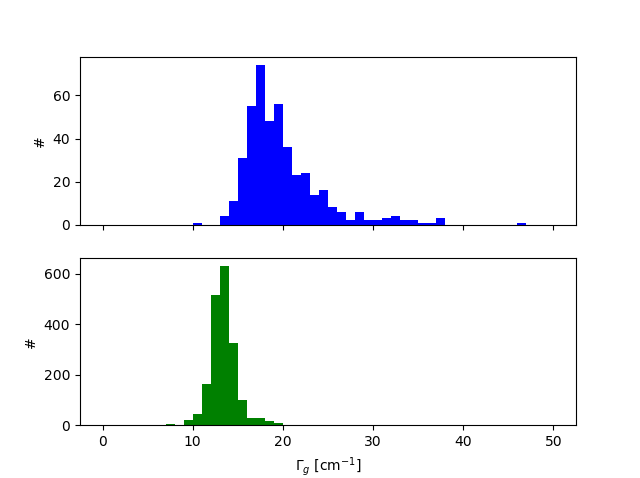
\includegraphics[scale=0.5]{Bilder/Laser/gammag_hist.png}
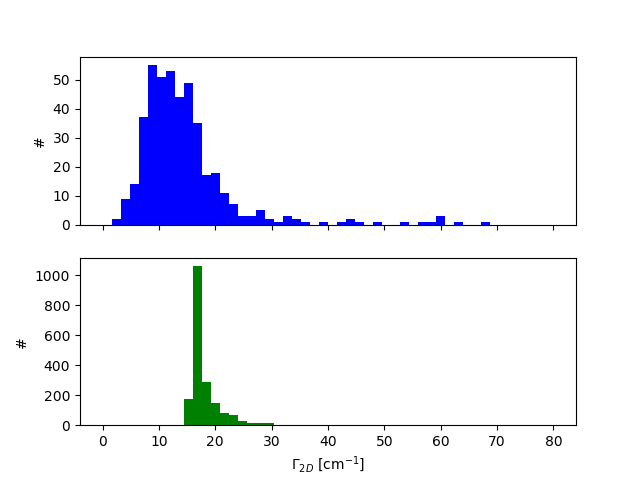
\includegraphics[scale=0.5]{Bilder/Laser/gamma2d_hist.png}
\caption{Distribution of the FWHD for the blue(top) and green(bottom) Laser. Right: $\Gamma_{g}$, left: $\Gamma_{2D}$.}
\label{fig:Laser_omega_hist}
\end{figure}





\end{document}